\documentclass[conference]{IEEEtran}
\IEEEoverridecommandlockouts
% The preceding line is only needed to identify funding in the first footnote. If that is unneeded, please comment it out.
\usepackage{cite}
\usepackage{amsmath,amssymb,amsfonts}
\usepackage{algorithmic}
\usepackage{graphicx}
\usepackage{textcomp}
\usepackage{xcolor}
\def\BibTeX{{\rm B\kern-.05em{\sc i\kern-.025em b}\kern-.08em
T\kern-.1667em\lower.7ex\hbox{E}\kern-.125emX}}
\newcommand\blfootnote[1]{%
\begingroup
\renewcommand\thefootnote{}\footnote{#1}%
\addtocounter{footnote}{-1}%
\endgroup
}
\usepackage{float}
\floatstyle{plaintop}
\restylefloat{table}

\usepackage{booktabs}
\usepackage{dcolumn}
\newcolumntype{d}[1]{D..{#1}}
\newcommand{\mc}[1]{\multicolumn{1}{c@{}}{#1}}

\begin{document}

\title{A Deep Learning Approach to Automatic Prosodic Segmentation in Untranscribed Discourse\\
}

\author{\IEEEauthorblockN{Nathan Roll}
\IEEEauthorblockA{\textit{University of California, Santa Barbara} \\
\texttt{nroll@ucsb.edu}}
\and
\IEEEauthorblockN{Dr. Calbert Graham}
\IEEEauthorblockA{\textit{University of Cambridge} \\
\texttt{crg29@cam.ac.uk}}

}

\maketitle

\begin{abstract}
Information in spoken language is determined by both the semantic meaning of words and the manner in which they are spoken, known as prosody. Prosodic units, also known as intonation units (IUs), are short phrases, each bound by a single tune, that play a role in both cognitive processing and speech synthesis. Despite applications in a variety of domains ranging from discourse analysis to synthetic speech generation, automatic IU identification remains unsolved. We propose a completely automated approach to the identification of prosodic boundaries utilizing a heuristic potential boundary reduction algorithm, input space compression, and an ensemble of CNN and RNN models, resulting in an F-score of 0.74.
\end{abstract}

\section{Introduction}
Humans are exceptional at recognizing patterns, even when they may be elusive computationally. Identification of intonation units (IUs) is no exception, as dozens of empirically abstract cues collectively comprise our perception of prosodic segments. Some of the most important are tune gestalt (unity of pitch/intonation contour), reset (return to a baseline pitch), silent pauses, anacrusis (rapid, unstressed syllables), and lag (lengthening of speech) \cite{b1}. We hypothesize that sufficiently complex computational models may be able to recognize some of these cues without the need for an accompanying lexical transcription.

Some attempts have already been made towards automatic segmentation and boundary detection in speech using a variety of methods. Semi-supervised Learning for Automatic Prosodic Event Detection Using Co-training Algorithm \cite{b2} achieves an F-score of 0.77 on a supervised labeled prosodic break detection task. In Automatic Detection of Prosodic Boundaries in Spontaneous Speech \cite{b3}, a variety of heuristic and theoretical models were able to achieve an F-score of 0.65 without the need for supervised training. Variances in segment definitions, input features (syntactic and/or acoustic), and corpus content (number of speakers, scripted or unscripted, etc.), however, make comparisons of results difficult.

We define boundaries as timestamps which occur at the beginning or end of an IU. A dynamic number of speakers means that multiple initial or end boundaries may occur sequentially in simultaneous speech examples. Successful identification of these boundaries lays the foundations for an automatic segmentation system while also helping us better understand prosody. Applications also exist in other domains, notably fluency assessment and synthetic speech generation \cite{b4} \cite{b5}.

Convolutional neural networks (CNNs) and recurrent neural networks (RNNs) are utilized for their distinct specializations. CNNs are designed for image recognition tasks– passing convolutional filters over groups of pixels or other filters repeatedly to determine which ones hold predictive power \cite{b6}. In contrast, RNNs excel at modeling temporal sequences. They attempt to generalize sequential relationships which may extend across an entire sample. Such an architecture may be able to identify segment-spanning features like tune, while underperforming CNNs in short-term signatures like pitch reset or vocal quality changes.


The framework proposed has the following advantages:
\begin{itemize}
\item Inferences can be made from audio files alone; transcript-reliant forced alignment is replaced by a heuristic algorithm.
\item Predictions are near-instantaneous.
\item Multiple relationships are considered in parallel.
\end{itemize}
\smallskip
For training and testing purposes, we use the Santa Barbara Corpus of Spoken American English (SBC), a collection of 60 discourse events spanning about 20 hours \cite{b7}. Included are stereo audio files (22,050 Hz) and manually generated IU-segmented transcripts with timestamps accurate to the nearest tenth of a second. A variety of demographic backgrounds (age, race, sex) are represented, with sensitive information removed in a manner which preserves pitch.
\smallskip
\section{Methods}
\subsection{Preprocessing}\label{AA}
The audio files in the Santa Barbara Corpus were reduced to a single channel through left-right averaging and downsampled to 8kHz. Given that boundaries must occur directly preceding or following a word, as IUs do not encompass peripheral pauses, mid-word or mid-pause samples did not need to be considered in the data. Also, a lack of precision (0.05s at 8kHz yields a potential error of 400 samples) must be accounted for. Forced alignment is an option, but this requires prior transcription and is relatively expensive computationally. \cite{b8}. Instead, we implement a maximum-recall algorithm to identify all potential IU boundaries \footnote{All code, including examples and descriptions, can be found in the project github: https://github.com/Nathan-Roll1/ProsodPy}:

\begin{enumerate}
\item Take the absolute value of given waveform
\item Compute the moving average over \emph{n} samples (\emph{n}=0.025s=200)
\item Subset every \emph{n}th value
\item Index local minima
\item Potential boundaries exist where minima separate speech above given threshold

\begin{figure}[htbp]
\centerline{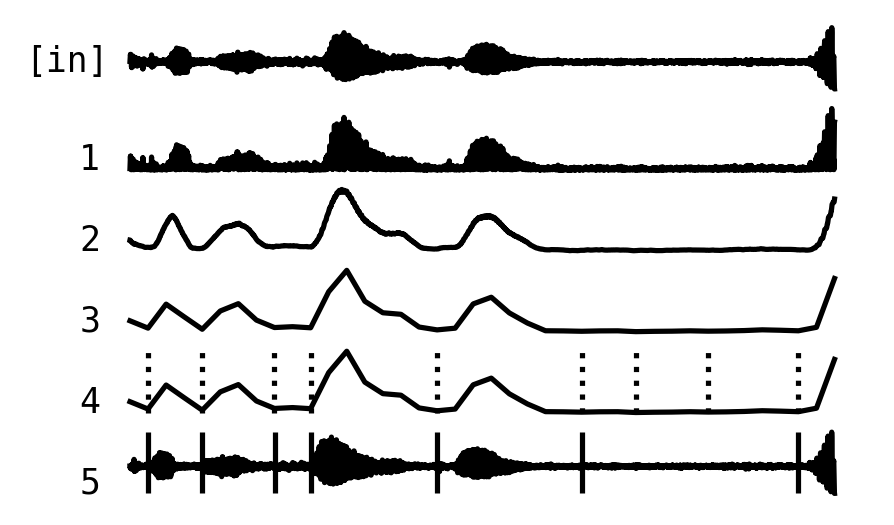
\includegraphics[width=75mm]{h_all.png}}
\caption{Boundary Heuristic Algorithm on SBC 32: 1.0s to 2.0s}
\label{fig}
\end{figure}
\end{enumerate}
Mel-frequency cepstral coefficients (MFCCs) are spectral transformations which maintain some pitch, intentity, and temporal information \cite{b9}. For each manually transcribed boundary and an equal number of randomly selected non-boundaries (identified by the heuristic), the first fifteen MFCCs were extracted with a hop length of 16 samples (0.002s) and a window size of 624 samples (0.078s) with a buffer of 512 frames (0.624s) on either side. To avoid precision loss due to padding, a minimal number of boundaries occurring at the beginning or end of the audio files were discarded. Each MFCC was normalized on its own axis by subtracting the mean and dividing by the standard deviation. A balanced dataset of 128,508 MFCC matrices and associated labels (true/false boundaries) form our train (80\%), test (10\%), and validation (10\%) sets.

The prior (preboundary), surrounding (boundary), and posterior (postboundary) featuresets within each MFCC are considered separately to explicitly match input sequences to boundaries. An additional 50\% subset of each is also considered (with the prefix “h\_”).


\begin{figure}[htbp]
\centerline{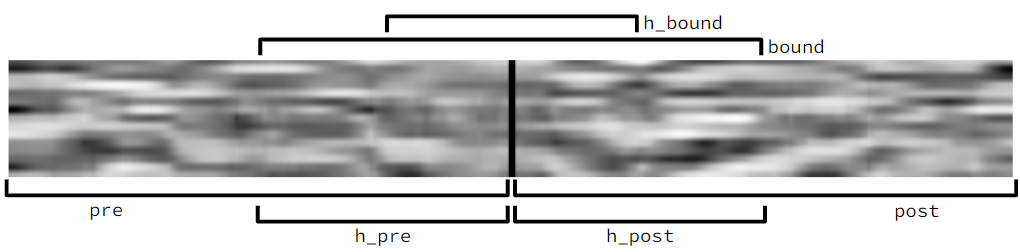
\includegraphics[width=90mm]{train_seg.png}}
\caption{MFCC-Extracted Featuresets}
\label{fig}
\end{figure}

Postboundary matrices are inverted on the temporal axis so that the sequence terminus corresponds to the boundary in question.


\subsection{Neural Networks}\label{AA}
The CNNs and RNNs are both trained using MSE loss, minimizing the squared distance between the floating point sigmoid outputs and the binary boundary classes. Due to inconsistencies during training, the CNN models utilize the stochastic gradient descent (SGD) optimizer while the RNNs use Adam \cite{b10}. The models which perform best on the validation data during training are checkpointed with a max epoch of 45.

CNN architecture:
\begin{center}
\begin{tabular}{ c }
Conv2d: 128 3x3 Filters; ReLU\\
Conv2d: 64 3x3 Filters; ReLU\\
2x2 Max Pooling\\
Flattening Layer\\
Dense: 8 Nodes; Tanh\\
20\% Dropout\\
Dense: 1 Node; Sigmoid
\end{tabular}
\end{center}

RNN architecture:
\begin{center}
\begin{tabular}{ c }
LSTM: 128 Units; Sigmoid\\
LSTM: 64 Units; Sigmoid\\
Dense: 32 Nodes; Tanh\\
20\% Dropout\\
Dense: 1 Node; Sigmoid
\end{tabular}
\end{center}

\subsection{Ensemble}\label{AA}
CNN and RNN outputs on the training data are regressed on boundary labels using an ordinary least squares (OLS) regression (fig. 3). This determines which models are significant, how they should be weighted, and acts as its own predictive model. \footnote{Models are trained on a remote Python 3.7.13 environment using tensorflow\cite{b11} and scikit-learn\cite{b12}}
\begin{figure}[htbp]
\centerline{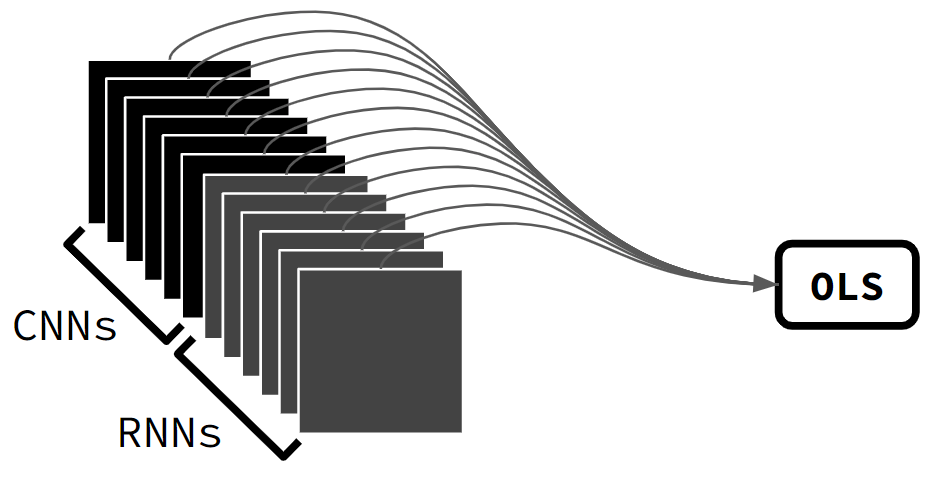
\includegraphics[width=60mm]{diagram_models.png}}
\caption{Ensemble Diagram}
\label{fig}
\end{figure}



\section{Results}
\subsection{Metrics}\label{AA}
We find that MFCC-based neural networks provide significant predictive power in the determination of IU boundaries. Furthermore, linear combinations of their outputs outperform any one individually.

The regression problem is transformed into one of classification by rounding the continuous outputs off at certain thresholds (\emph{t}). Intermediate steps were evaluated using MSE and $r^2$, while the binary categorical results of rounding are measured in terms of F-score and accuracy. F-score is particularly informative in the realm of cross-model evaluation and precision/recall balancing.

Accuracy and F-score reach their optima at different thresholds (fig. 4), with \emph{t}=0.5 achieving the maximum accuracy of 72.36\% (Table I), and \emph{t}=0.37 achieving the maximum F-score of 73.88\% (Table II) on unseen data. A baseline of all positive predictions is included for reference. Preboundary features, specifically MFCCs one second leading up to a potential boundary, are the most valuable individually at predicting whether or not it truly marks the start/end of an IU.

\begin{figure}[htbp]
\centerline{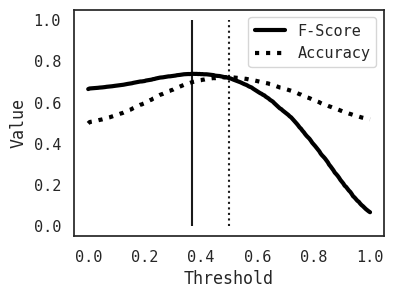
\includegraphics[width=70mm]{f1_acc.png}}
\caption{F-Score reaches its maximum at a threshold of 0.37}
\label{fig}
\end{figure}



\begin{table}
\caption{Performance Metrics (\emph{t}=0.5)}
\smallskip
\begin{center}
\begin{tabular}{lrrrr}
\toprule
{} & F1 & Precision & Recall & Accuracy $\Downarrow$\\
\midrule
\bf{OLS} & \bf{0.719} & \bf{0.728} & \bf{0.709} & \bf{0.724} \\
pre\_rnn & 0.683 & 0.707 & 0.660 & 0.695 \\
h\_pre\_rnn & 0.679 & 0.693 & 0.666 & 0.687 \\
h\_bound\_rnn & 0.680 & 0.660 & 0.701 & 0.671 \\
bound\_cnn & 0.648 & 0.676 & 0.622 & 0.663 \\
h\_bound\_cnn & 0.657 & 0.655 & 0.659 & 0.658 \\
h\_pre\_cnn & 0.645 & 0.636 & 0.655 & 0.642 \\
pre\_cnn & 0.628 & 0.641 & 0.615 & 0.637 \\
post\_rnn & 0.614 & 0.650 & 0.582 & 0.636 \\
post\_cnn & 0.591 & 0.602 & 0.580 & 0.600 \\
bound\_rnn & 0.556 & 0.562 & 0.551 & 0.562 \\
h\_post\_rnn & 0.530 & 0.566 & 0.499 & 0.560 \\
h\_post\_cnn & 0.537 & 0.553 & 0.522 & 0.552 \\
\emph{baseline} & \emph{0.665} & \emph{0.498} & \emph{1.000} & \emph{0.498} \\
\bottomrule
\end{tabular}

\end{center}
\end{table}

\begin{table}
\caption{Performance Metrics (\emph{t}=0.37)}
\smallskip
\begin{center}
\begin{tabular}{lrrrr}
\toprule
{} & F1 $\Downarrow$& Precision & Recall & Accuracy \\
\midrule
\bf{OLS} & \bf{0.739} & \bf{0.650} & \bf{0.855} & \bf{0.699} \\
pre\_rnn & 0.717 & 0.622 & 0.845 & 0.668 \\
h\_pre\_rnn & 0.709 & 0.605 & 0.854 & 0.650 \\
h\_bound\_rnn & 0.703 & 0.595 & 0.859 & 0.639 \\
bound\_cnn & 0.694 & 0.607 & 0.812 & 0.644 \\
h\_bound\_cnn & 0.693 & 0.586 & 0.849 & 0.627 \\
h\_pre\_cnn & 0.683 & 0.566 & 0.859 & 0.603 \\
post\_rnn & 0.681 & 0.565 & 0.857 & 0.601 \\
pre\_cnn & 0.679 & 0.573 & 0.833 & 0.608 \\
post\_cnn & 0.666 & 0.536 & 0.879 & 0.561 \\
h\_post\_rnn & 0.665 & 0.498 & 1.000 & 0.498 \\
bound\_rnn & 0.665 & 0.498 & 1.000 & 0.498 \\
\emph{baseline} & \emph{0.665} & \emph{0.498} & \emph{1.000} & \emph{0.498} \\
h\_post\_cnn & 0.663 & 0.499 & 0.989 & 0.500 \\
\bottomrule
\end{tabular}

\end{center}
\end{table}


Higher predictions lead to a higher likelihood of a true boundary and vice-versa (fig. 5).

\begin{figure}[htbp]
\centerline{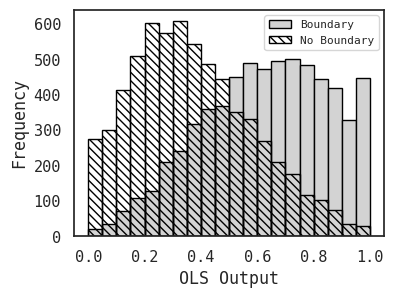
\includegraphics[width=70mm]{boundary_hist.png}}
\caption{OLS-predicted values versus binary truth}
\label{fig}
\end{figure}

\subsection{Implementation}\label{AA}

Processing time through the proposed framework is linear [O(n)], requiring 0.052 seconds per second of input audio on our system.\footnote{This does not include environment initialization or resampling and may take longer without access to GPU resources.}Given an imbalance of true and false boundaries in naturally occurring discourse (there are many more of the latter), we suggest using a threshold of 0.37 instead of 0.5 (fig. 6). Please see our github\footnote{https://github.com/Nathan-Roll1/ProsodPy} for specific implementation instructions.

\begin{figure}[htbp]
\centerline{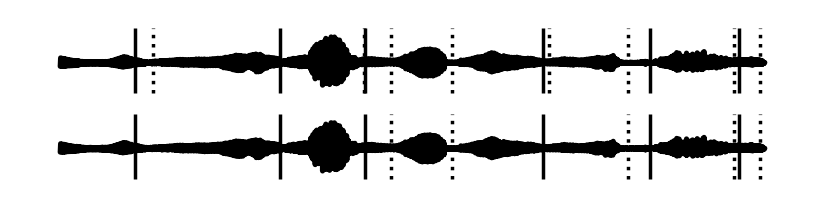
\includegraphics[width=90mm]{implementation.png}}
\caption{Output of entire framework (dotted) versus actual transcription (solid)  top: \emph{t}=0.37,  bottom: \emph{t}=0.5 (SBC 32: 2s to 4s)}
\label{fig}
\end{figure}


\section{Conclusion}
MFCC transformations of audio data are powerful predictors of intonation unit boundaries. There still, however, remains unexplained variation. A theoretical accuracy limit of 80\% (the threshold of inter-human agreement) \cite{b3} leaves much to be desired from an automatic prosodic segmentation system. We expect that hyperparameter tuning, expanded input data, and more powerful models will improve the results reported in this work.


\section*{Acknowledgments}

We thank Dr. John Du Bois (University of California, Santa Barbara), Dr. Tirza Biron (Weizmann Institute of Science), and the University of Cambridge.

\begin{thebibliography}{00}
\bibitem{b1} Du Bois JW, Cumming S, Schuetze-Coburn S, Paolino D. Discourse transcription, Santa Barbara Papers in Linguistics vol. 4. 1992.
\bibitem{b2} Jeon, Je Hun \& Liu, Yang. (2009). Semi-supervised Learning for Automatic Prosodic Event Detection Using Co-training Algorithm. 540-548. 10.3115/1690219.1690222.
\bibitem{b3} Biron T, Baum D, Freche D, Matalon N, Ehrmann N, Weinreb E, et al. (2021) Automatic detection of prosodic boundaries in spontaneous speech. PLoS ONE 16(5): e0250969. https://doi.org/10.1371/journal.pone.0250969
\bibitem{b4} Kuhn, Melanie \& Schwanenflugel, Paula \& Meisinger, Elizabeth. (2010). Aligning theory and assessment of reading fluency: Automaticity, prosody, and definitions of fluency. Reading Research Quarterly. 45. 232-253.
\bibitem{b5} Julia Hirschberg, Communication and prosody: Functional aspects of prosody, Speech Communication, Volume 36, Issues 1–2, 2002, Pages 31-43,ISSN 0167-6393, https://doi.org/10.1016/S0167-6393(01)00024-3.
\bibitem{b6} O. Abdel-Hamid, A. Mohamed, H. Jiang, L. Deng, G. Penn and D. Yu, "Convolutional Neural Networks for Speech Recognition," in IEEE/ACM Transactions on Audio, Speech, and Language Processing, vol. 22, no. 10, pp. 1533-1545, Oct. 2014, doi: 10.1109/TASLP.2014.2339736.
\bibitem{b7} Du Bois, John W., Wallace L. Chafe, Charles Meyer, Sandra A. Thompson, Robert Englebretson, and Nii Martey. 2000-2005. Santa Barbara corpus of spoken American English, Parts 1-4. Philadelphia: Linguistic Data Consortium.
\bibitem{b8} Moreno, Pedro \& Joerg, Christopher \& Thong, Jean-Manuel \& Glickman, Oren. (1998). A recursive algorithm for the forced alignment of very long audio segments. 10.21437/ICSLP.1998-603.
\bibitem {b9} P. Mermelstein (1976), "Distance measures for speech recognition, psychological and instrumental," in Pattern Recognition and Artificial Intelligence, C. H. Chen, Ed., pp. 374–388. Academic, New York.
\bibitem {b10} Kingma, Diederik P., and Jimmy Ba. "Adam: A method for stochastic optimization." arXiv preprint arXiv:1412.6980 (2014).
\bibitem {b11} Martín Abadi et al. TensorFlow: Large-scale machine learning on heterogeneous systems, 2015. Software available from tensorflow.org.
\bibitem {b12}Scikit-learn: Machine Learning in Python, Pedregosa et al., JMLR 12, pp. 2825-2830, 2011
\end{thebibliography}
\end{document}


